\section{Multivariate linear regression}
\subsection{Multiple features - multiple variables}
When an output does not depend only on ONE variable (input) but also on multiple variables. Each variable (input) is called as a feature.
\textbf{Notation}
\begin{itemize}
	\item n = number of features  (in table \ref{tab:ex_multiple_features} is number of column = 4)
	\item m = number of an training example (number of row = m)
	\item $x^{(i)}$ = input (features) of $i^{th}$ training example
	\item $x^{i}_j$ = value of feature j in $i^{th}$ training example
\end{itemize}

Example: Let's say housing price depends on 4 features as shown in Tab. \ref{tab:ex_multiple_features}
\begin{table}[h]
	\centering
	\begin{tabular}{|c|c|c|c|c|}
		\toprule 
		\textbf{Size} & \textbf{\# of bedrooms} & \textbf{\# of floors} & \textbf{Age of home} & \textbf{Price} \\
		 $x_1$ &$x_2$& $x_3$ & $x_4$ & y  \\
		\midrule 
		2104 	& 5 	& 1 & 45 & 460 \\
		123 	 & 1 	 & 3 & 32 & 232 \\
		3211 	 & 4  	& 4 & 32 & 432 \\
		...  & ... & ... & ... & ... \\
		\bottomrule
	\end{tabular}
\caption{An example of multiple features}
\label{tab:ex_multiple_features}
\end{table}

Saying: $x^{(1)} = \begin{bmatrix}
2014 \\5 \\ 1\\ 45 \\ 460 \\
\end{bmatrix}$  $\in \Re^{n}$ \\
$x^{(1)}$ is the $1^{st}$ training set, it includes all inputs (features) of the $1^{st}$ training set.\\

\textbf{Linear regression with multiple variables is also known as "multivariate linear regression"}
%%%%%%%%%%%%%%%%%%%%%%%%%%%%%%%%%%%%%%%%%%%%%
%%%%%%%%%%%%%%%%%%%%%%%%%%%%%%%%%%%%%%%%%%%%%
\subsection{Hypothesis}
The hypothesis for multiple variables or multiple feature will be expressed as:
\begin{equation*}
\begin{aligned}
h_{\theta} &= \theta_0 + \theta_1 x_1 + \theta_2 x_2 + \theta_3 x_3 + ... + \theta_n x_n \\ \\
\end{aligned}
\end{equation*}

Lets define $x_0 = 1$ or ($x^{(i)}_0 = 1$, which means all training example of feature 0 equal to 1.
Hence, 
\begin{equation}
\begin{aligned}
h_{\theta} &= \theta_0 x_0 + \theta_1 x_1 + \theta_2 x_2 + \theta_3 x_3 + ... + \theta_n x_n \\ \\
\end{aligned}
\end{equation}

In addition, substitue:
\begin{equation}
X = \begin{bmatrix}
			x_{0} \\
			x_{1} \\
			x_{2} \\
			\vdots \\
			x_{n}
		\end{bmatrix} \in \Re{^{n+1}} 	\hspace*{10mm}	
\theta = \begin{bmatrix}
			\theta_{0} \\
			\theta_{1} \\
			\theta_{2} \\
			\vdots \\
			\theta_{n+1} 
\end{bmatrix}	\in \Re{^{n}}
\end{equation}

Finally, \textbf{multivariate linear regression} is expressed as
\begin{equation}
\begin{aligned}
h_{\theta} &= \theta^\intercal X\\
h_{\theta} &= \left[\theta_{0}, \theta_{1}, \theta_{2}, \cdots, \theta_{n+1} \right] \cdot \begin{bmatrix}
				x_{0} \\
				x_{1} \\
				x_{2} \\
				\vdots \\
				x_{n}
				\end{bmatrix}
\end{aligned}
\end{equation}

where:
\begin{itemize}
	\item X is a vector of inputs or features
	\item $\theta^\intercal$ is a transpose of the column matrix $\theta$
\end{itemize}
\subsection{Gradient Descent for multiple variables}
\subsubsection{Cost function}
Renote: The \textbf{cost function} is a function of $\theta$ \\
\textbf{The previous version} for single variable:
\begin{equation*}
J(\theta_0, \theta_1) = \dfrac {1}{2m} \displaystyle \sum _{i=1}^m \left ( \hat{y}^{(i)}- y^{(i)} \right)^2 = \dfrac {1}{2m} \displaystyle \sum _{i=1}^m \left (h_\theta (x^{(i)}) - y^{(i)} \right)^2
\end{equation*}

where:
\begin{itemize}
	\item $\hat{y}^{(i)}$ is the hypothesis value of output corresponding an input in the $i^{th}$ training example
	\item $y^{(i)}$ is the actual output in the $i^{th}$ training example
	\item $x^{(i)}$ is the input in the $i^{th}$ training example
	\item $\theta_0, \theta_1$ are coefficients or parameters
\end{itemize}

The same function is applied for multivariate linear regression. But, we have multiple variables \\
$=>$ MUST have multiple coefficients $\theta$ \\\\

\textbf{The new version:}
\begin{equation*}
J(\theta_0, \theta_1, ..., \theta_n) = \dfrac {1}{2m} \displaystyle \sum _{i=1}^m \left ( \hat{y}^{(i)}- y^{(i)} \right)^2 = \dfrac {1}{2m} \displaystyle \sum _{i=1}^m \left (h_\theta (x^{(i)}) - y^{(i)} \right)^2
\end{equation*}

\begin{align*} 
	& \text{repeat until convergence:} \; \lbrace \\ \; 
	& \theta_0 := \theta_0 - \alpha \frac{1}{m} \sum\limits_{i=1}^{m} (h_\theta(x^{(i)}) - y^{(i)}) \cdot x_0^{(i)} \\ \; 
	& \theta_1 := \theta_1 - \alpha \frac{1}{m} \sum\limits_{i=1}^{m} (h_\theta(x^{(i)}) - y^{(i)}) \cdot x_1^{(i)} \\ \; 
	& \theta_2 := \theta_2 - \alpha \frac{1}{m} \sum\limits_{i=1}^{m} (h_\theta(x^{(i)}) - y^{(i)}) \cdot x_2^{(i)} \\
	& \cdots \\ \rbrace 
\end{align*}

\begin{figure}[h]
	\centering
	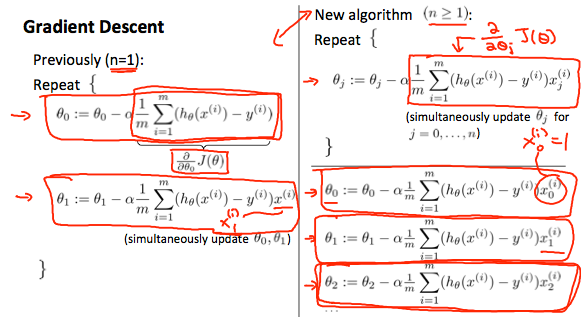
\includegraphics[ clip, scale=0.5]{img/gradient_descent_gen.png}
	\caption{ Difference between Univariate and Multivariate version}
\end{figure}

\subsection{Notes to improve runtime of Gradient Descent}
\subsubsection{Scaling feature}
Scaling features is a MUST before running algorithm because of the fact:
\begin{itemize}
	\item The longer range of a feature, the slower the cost function converges
\end{itemize}

Putting all features in a same scale helps reducing runtimes of the algorithms.\\

\textbf{What a contour look like if using feature with different scales?}
\begin{itemize}
	\item The thinner side of contour is the $\theta$ of the longer-range feature 
	\item The wider side of contour is the $\theta$ of the shorter-range feature
\end{itemize}
\hspace*{5mm} Or we can say: \textit{a longer range feature has a shorter range of $\theta$}\\
Scaling feature makes contour more likes a circles\\

\textbf{Example:} \\
The housing price depends on 2 features: the area and the number of floors. Lets say 
\begin{itemize}
	\item Area varies from 50 $m^2$ - 200 $m^2$
	\item Number of floors varies from 1 - 5
\end{itemize}

Scaling feature means instead of using a feature with a range (50 - 200) and a feature with a range (1 - 5) as inputs of gradient descent algorithm. We uses a scaling feature with a range ($\displaystyle\frac{50}{200}$ -  $\displaystyle\frac{200}{200}$) or (0.25 - 1) and  a scaling feature with a range (0.2 - 1). \\

\textbf{Each feature can have different scaling factors} \\ \\
\textbf{RULES for scaled range}
\begin{itemize}
	\item $\left[-3,  +3\right]$ is OK, any larger: BAD
	\item $\left[-\displaystyle\frac{1}{3}, +\displaystyle\frac{1}{3}\right]$ is OK, any smaller: BAD
\end{itemize}

\subsubsection{Mean normalization}
Aim of normalizing the mean is to bring the mean of "feature's range" close to zero. \\
Take a feature $x_j$ and replace it by:\\
\begin{equation*}
\frac{x_j - \mu_j}{\sigma_j}
\end{equation*}

where:
\begin{itemize}
	\item $\mu_j$ is mean or average of values of feature $j^{th}$
	\item $\sigma_j$ is the standard deviation of feature $j^{th}$, it is calculated as (max - min)
\end{itemize}

\textbf{Example:}\\
Let say size is a feature that affects the housing price. In training examples, its range is from 100 - 180. The mean of size feature is 140 and the standard deviation is 80. \\
The feature that we use in hypothesis is $\displaystyle\frac{x_j - 140}{80}$

\subsubsection{Learning Rate $\alpha$}
This section explains how we choose a suitable $\alpha$ \\ \\
\textbf{Tool for checking the Gradient Descent working or not $\alpha$} \\
Using plot of min($J(\theta)$) vs No. of iteration\\ 
\begin{figure}[h]
	\centering
	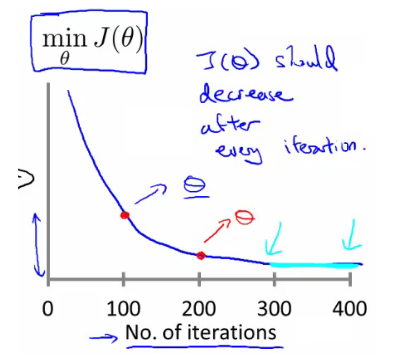
\includegraphics[ clip, scale=0.61]{img/plot_no_iter.png}
	\caption{ Plot for checking Gradient Descent }
	\label{fig:checkingplot}
\end{figure}

\textbf{PRINCIPAL:  J($\theta$) decreases after every iteration}
\begin{itemize}
	\item IF: decreasing slowly, then need to increase $\alpha$
	\item IF: non-decreasing, then need to reduce $\alpha$
\end{itemize}

Typically, a the process for alpha selection 
\begin{itemize}
	\item Try a range of alpha values
	\item Plot J($\theta$) vs number of iterations for each version of alpha
	\item Go for roughly threefold increases: 0.001, 0.003, 0.01, 0.03. 0.1, 0.3
\end{itemize}

%%%%%%%%%%%%%%%%%%%%%%%%%%%%%%%%%%%%%%%%%%%%%%%%%
%%%%%%%%%%%%%%%%%%%%%%%%%%%%%%%%%%%%%%%%%%%%%%%%%
\subsection{Features vs Polynomial Regression}
\begin{itemize}
	\item DO NOT need to use all features (since some features are correlated), there are algorithms to choose suitable features
	\item Sometimes, form of actual data (such as: price vs size) does not look like a linear funtion, we have to use POLYNOMIAL REGRESSION
\end{itemize}

\subsubsection{Features}
We can \large{\textbf{create a new feature}} \\[1.5ex]
Example\\
In house price prediction,
Two features:
\begin{itemize}
	\item Frontage ($x_1$) - width of the plot of land along road 
	\item Depth ($x_2$)- depth away from road 
\end{itemize}

Might decide that an important feature is the land area. \\
So, create a new feature (may be a better indicator), area ($x_3)$ = frontage * depth \\
Now, the new model is:
$$h(\theta) = \theta_0 + \theta_1 x_3$$

\subsubsection{Polynomial Regression}
\begin{figure}[h]
	\centering
	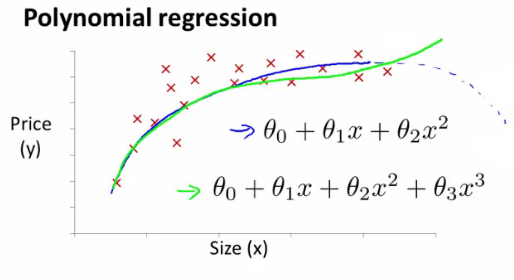
\includegraphics[ clip, scale=0.81]{img/poly_regression.png}
	\caption{Choosing a polynomial to express actual relationship}
	\label{fig:poly_regression}
\end{figure}

How do we create the model to this data? \\
Having a set of:
\begin{align*}
x_1 &= x \\
x_2 &= x^2 \\
x_3 &= x^ 3
\end{align*}

By selecting the features like this and applying the linear regression algorithms you can do polynomial regression. \\
Remember, feature scaling becomes even more important here. \\

%%%%%%%%%%%%%%%%%%%%%%%%%%%%%%%%%%%%%%%%%%%%%%%%%
%%%%%%%%%%%%%%%%%%%%%%%%%%%%%%%%%%%%%%%%%%%%%%%%%
%%%%%%%%%%%%%%%%%%%%%%%%%%%%%%%%%%%%%%%%%%%%%%%%%
%%%%%%%%%%%%%%%%%%%%%%%%%%%%%%%%%%%%%%%%%%%%%%%%%
%%%%%%%%%%%%%%%%%%%%%%%%%%%%%%%%%%%%%%%%%%%%%%%%%
%%%%%%%%%%%%%%%%%%%%%%%%%%%%%%%%%%%%%%%%%%%%%%%%%
%%%%%%%%%%%%%%%%%%%%%%%%%%%%%%%%%%%%%%%%%%%%%%%%%
%%%%%%%%%%%%%%%%%%%%%%%%%%%%%%%%%%%%%%%%%%%%%%%%%
\section{NEW ALGORITHM: Analytically method to compute theta}
\subsection{Normal equation}
Formula: \\
\begin{equation*}
	\theta = (X^T X)^{-1}X^T y
	\label{eq:normaleq}
\end{equation*}

\begin{figure}[h]
	\centering
	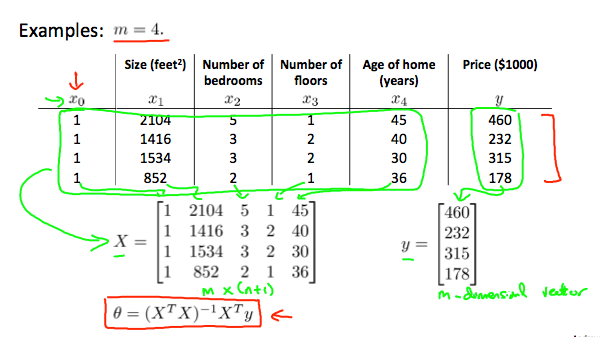
\includegraphics[ clip, scale=0.70]{img/normal_equation_ex.png}
\end{figure}

Gradient Descent: Finding value of $\theta$ for getting minimal value of the cost function by perform multiple iterations. \\
Normal equation: we will minimize J by explicitly taking its derivatives with respect to the $\theta^{(j)}$, and setting them to zero. This allows us to find the optimum theta without iteration. \\

\textbf{There is no need to do feature scaling with the normal equation}

The following is a comparison of gradient descent and the normal equation:
\begin{table}[h]
	\centering
	\begin{tabular}{|c|c|}
		\toprule 
	Gradient Descent &	Normal Equation \\ \midrule
	Need to choose alpha &	No need to choose alpha \\
	Needs many iterations &	No need to iterate \\
	O (k$n^2$)	& O ($n^3$), need to calculate inverse of $X^TX$ \\
	Works well when n is large &	Slow if n is very large \\
	\bottomrule
\end{tabular}
\end{table}

\textbf{n: number of features}\\
To be specific, n $>$ 10000 $=>$ should go with an iterative approach

\subsection{Normal Equation Noninvertibility}
As be described in Eq. \ref{eq:normaleq}; we need to do inverse operation of $(X^TX)^{-1}$. But in some cases, inverting is impossible. \\
Lets find out what are the causes of this problem:
\begin{itemize}
	\item Redundant features, where two features are very closely related (i.e. they are linearly dependent)
	\item Too many features (e.g. m $\leq$ n). In this case, delete some features or use "regularization" (to be explained in a later lesson).
\end{itemize}

\textbf{NOTE:} \\
In octave, using the 'pinv' function rather than 'inv.' Since the 'pinv' function will give you a value of $\theta$ even if $X^TX$ is not invertible.

\section{Practical part}
\subsection{Octave and Matlab}
Lets check how gitignore works
